\documentclass[11pt, a4paper]{article}

% --- Packages ---
\usepackage[utf8]{inputenc}
\usepackage[T1]{fontenc}
\usepackage{mathptmx}
\usepackage{graphicx}
\usepackage[margin=0.8in]{geometry}
\usepackage{xcolor}
\usepackage{titlesec}
\usepackage{enumitem}
\usepackage{float}
\usepackage{booktabs}
\usepackage{multirow}
\usepackage{array}
\usepackage{url}

\graphicspath{{../figures/}}

% --- Amrita Colors ---
\definecolor{amritaMaroon}{HTML}{A4123F}

% --- Title & Section Formatting ---
\titlespacing*{\section}{0pt}{12pt}{4pt}
\titlespacing*{\subsection}{0pt}{8pt}{3pt}
\titleformat{\section}{\large\bfseries\color{amritaMaroon}}{\thesection}{0.8em}{}
\titleformat{\subsection}{\normalsize\bfseries\color{amritaMaroon}}{\thesubsection}{0.6em}{}

\pagestyle{plain}

\begin{document}

\noindent
\begin{minipage}{\textwidth}
    \centering
    {\Large \textbf{\textcolor{amritaMaroon}{
    AMRITA VISHWA VIDYAPEETHAM \\
    SCHOOL OF COMPUTING \\
    DEPARTMENT OF COMPUTER SCIENCE AND ENGINEERING \\
    }}}
    \vspace{0.2cm}
    {\large \textbf{Court-Calibrated Group Activity Recognition for Volleyball Team Behaviour Analysis Using Monocular Video}} \\[0.1cm]
    \textbf{23CSE498 -- Project Phase II (External Review)} \quad | \quad \textbf{Team Number: 56} \\
    \today
\end{minipage}

\vspace{0.3cm}
\hrule
\vspace{0.3cm}

\noindent
\begin{center}
    \renewcommand{\arraystretch}{1.45}
    \setlength{\tabcolsep}{6pt}
    \begin{tabular}{|l|p{4.8cm}|p{4.6cm}|p{3.2cm}|}
        \hline
        \multicolumn{2}{|c|}{\textbf{Team Members}} & \textbf{Project Guide} & \textbf{Project Type} \\
        \hline
        \small CB.SC.U4CSE23415 & \small G. Bharath Chandra &
        \multirow{5}{=}{\raggedright \small \textbf{Dr. Divya Singh} \newline \textit{Assistant Professor, \newline Dept. of CSE}} &
        \multirow{5}{=}{\raggedright \small \textbf{Type 2} \newline Application-Based Project} \\ \cline{1-2}
        \small CB.SC.U4CSE23420 & \small K. Surya Sekhar & & \\ \cline{1-2}
        \small CB.SC.U4CSE23425 & \small Keshavramprakash D. & & \\ \cline{1-2}
        \small CB.SC.U4CSE23453 & \small U. Yeshwanth Kumar Reddy & & \\ \cline{1-2}
        \small CB.SC.U4CSE23768 & \small V. Punith Sai & & \\
        \hline
    \end{tabular}
\end{center}
\vspace{0.2cm}

\section{Abstract}
\noindent
Volleyball coaches usually study match videos by hand to see how their team moves together. This takes a long time, and different people can judge the same rally differently. This project is a web application that does this automatically from an ordinary match video recorded with one camera. The user uploads a video and chooses the part to analyse. The system first checks that the video shows a volleyball court with players. It then finds and follows every player and the ball, separates the two teams, and studies how the near-side team moves and positions itself around the ball. A trained machine-learning model then names the team's tactic for every second of play: Coordinated Attack, Coordinated Defense, Delayed Support or Spacing Breakdown. The user receives an annotated video, a timed tactic report, a list of the opponent's serves, spikes and blocks, and short example clips. The application is complete and works end to end on a laptop with a graphics card, and all functional tests passed. On match videos the model had never seen, it named the correct tactic 63.7\% of the time, compared with 39.0\% for simple guessing.

\section{Problem Definition \& Requirement Analysis}

\subsection{Problem Statement, Context \& Target Users}
\begin{itemize}[noitemsep, topsep=2pt]
    \item \textbf{Problem Definition:} Coaches and analysts watch long match recordings to judge how a team attacks, defends and covers the court. Doing this by hand takes hours for each match, and two people can judge the same rally differently.
    \item \textbf{Target Users \& Stakeholders:} Volleyball coaches, performance analysts and players at clubs and colleges, who usually have only one camera and no special tracking equipment.
    \item \textbf{Existing Limitations:} Existing scouting tools need a person to watch the match and type in every event. Research methods for recognising group activities \cite{zhang2024bicausal,ibrahim2016} need player positions marked by hand, so they cannot be used directly on a normal match video.
    \item \textbf{Application Objectives:}
    \begin{enumerate}[noitemsep, topsep=2pt]
        \item Take an ordinary match video and produce results without any manual marking.
        \item Name the near-side team's tactic for every second of play, and check the accuracy on match videos the model has never seen.
        \item Provide everything through an easy web application with input checks, a live progress bar and clear messages.
    \end{enumerate}
\end{itemize}

\subsection{Functional \& Non-Functional Requirements}
\begin{table}[H]
    \centering
    \footnotesize
    \renewcommand{\arraystretch}{1.25}
    \begin{tabular}{|c|p{3.0cm}|p{9.2cm}|}
        \hline
        \textbf{Req. ID} & \textbf{Category} & \textbf{Requirement Specification} \\
        \hline
        FR-1 & Functional & Upload a match video (MP4, MOV, AVI, MKV, WebM) and choose the part to analyse. \\
        \hline
        FR-2 & Functional & Find and track players and the ball; give the near-side team one of 4 tactics for every second of play. \\
        \hline
        FR-3 & Functional & Show an annotated video and give downloadable reports: tactic timeline and opponent SERVE / SPIKE / BLOCK. \\
        \hline
        FR-4 & Functional & Keep a list of each user's past analyses. \\
        \hline
        NFR-1 & Non-Functional & Refuse wrong or non-volleyball files early with a clear message; show live progress while the video is being analysed. \\
        \hline
        NFR-2 & Non-Functional & Run on a normal laptop with a graphics card (NVIDIA RTX 3050); needs only one camera, no sensors or wearables. \\
        \hline
    \end{tabular}
    \caption{Summary of Application Functional and Non-Functional Requirements}
\end{table}

\section{Application Architecture \& Solution Design}

\subsection{End-to-End Application Architecture}
\noindent
Figure 1 shows how the application works, from upload to result. (1) The coach opens the website and uploads a match video. (2) The web page sends the video to the server in small parts and shows an upload progress bar. (3) The server checks that the file is a real video and that a volleyball court with players is visible, then places the job in a waiting line (queue). (4) The video is saved, and a record of the job is stored in the database. (5) A worker picks up one job at a time and starts the analysis. (6) The analysis engine finds the players and the ball, follows them through the video, and the trained model names the tactic for each second. (7) The finished video, reports and clips are saved and shown on the Results page. Figure 2 shows the steps inside the analysis engine.

\begin{figure}[H]
    \centering
    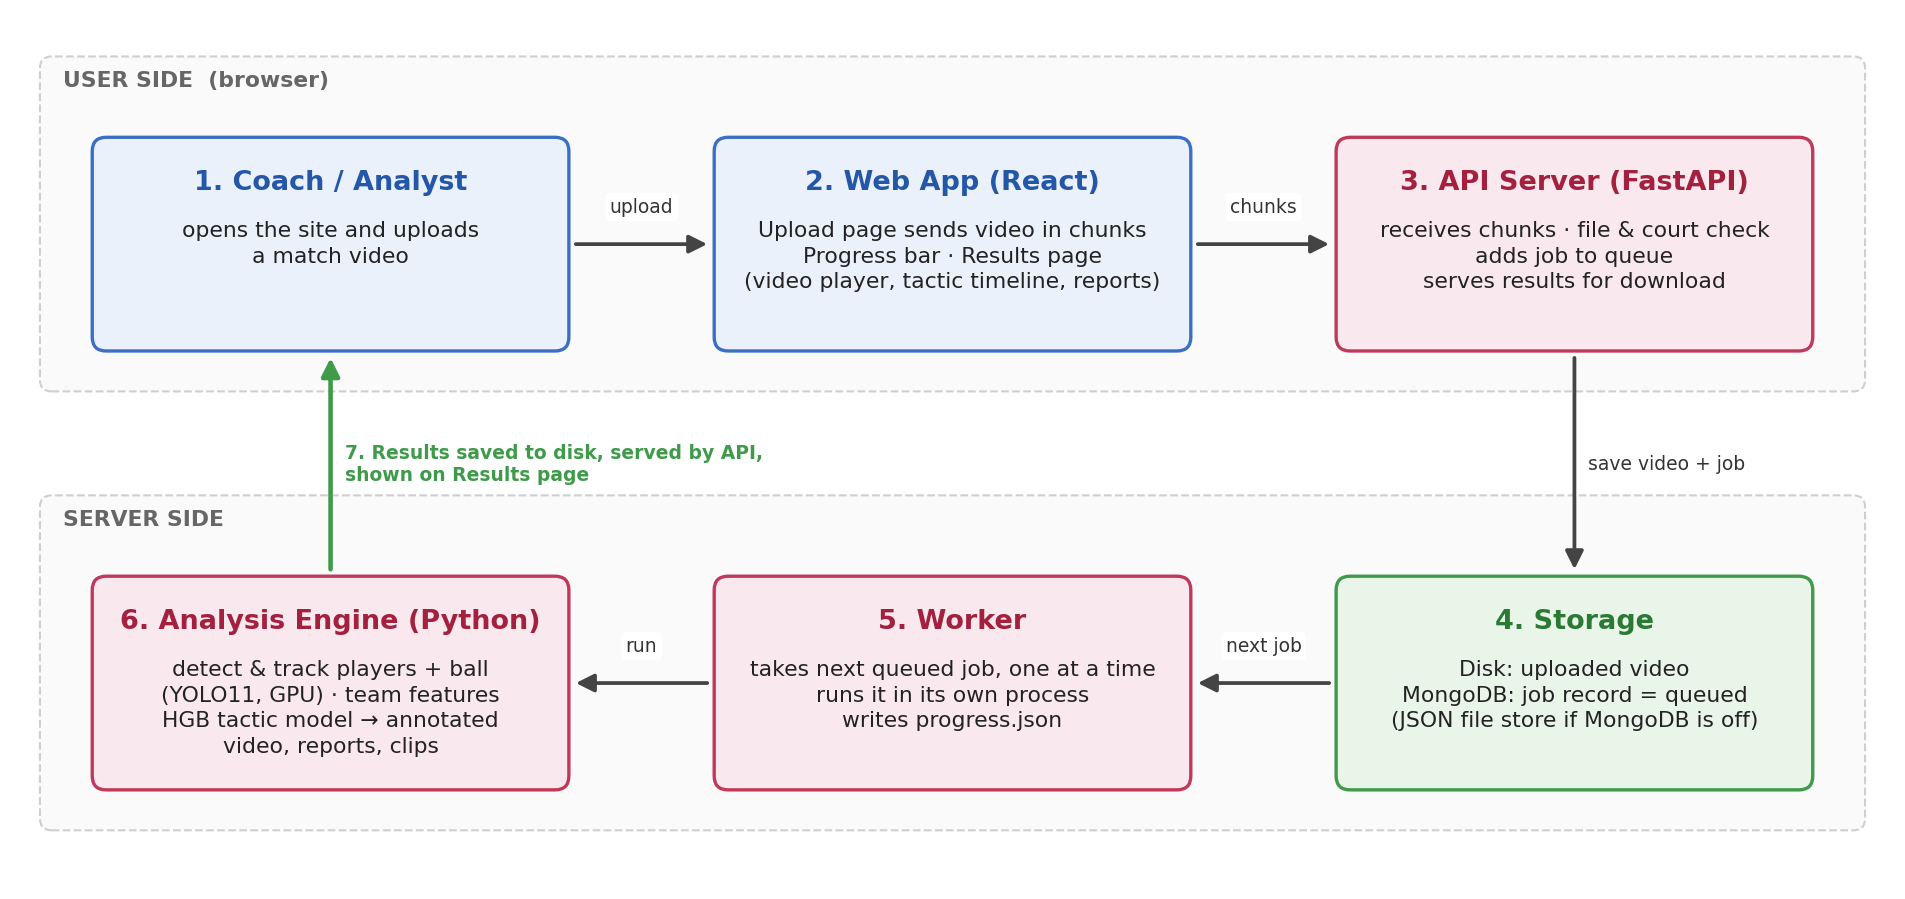
\includegraphics[width=\textwidth]{web_flow_loop.png}
    \caption{End-to-End Application Architecture and Workflow}
\end{figure}

\begin{figure}[H]
    \centering
    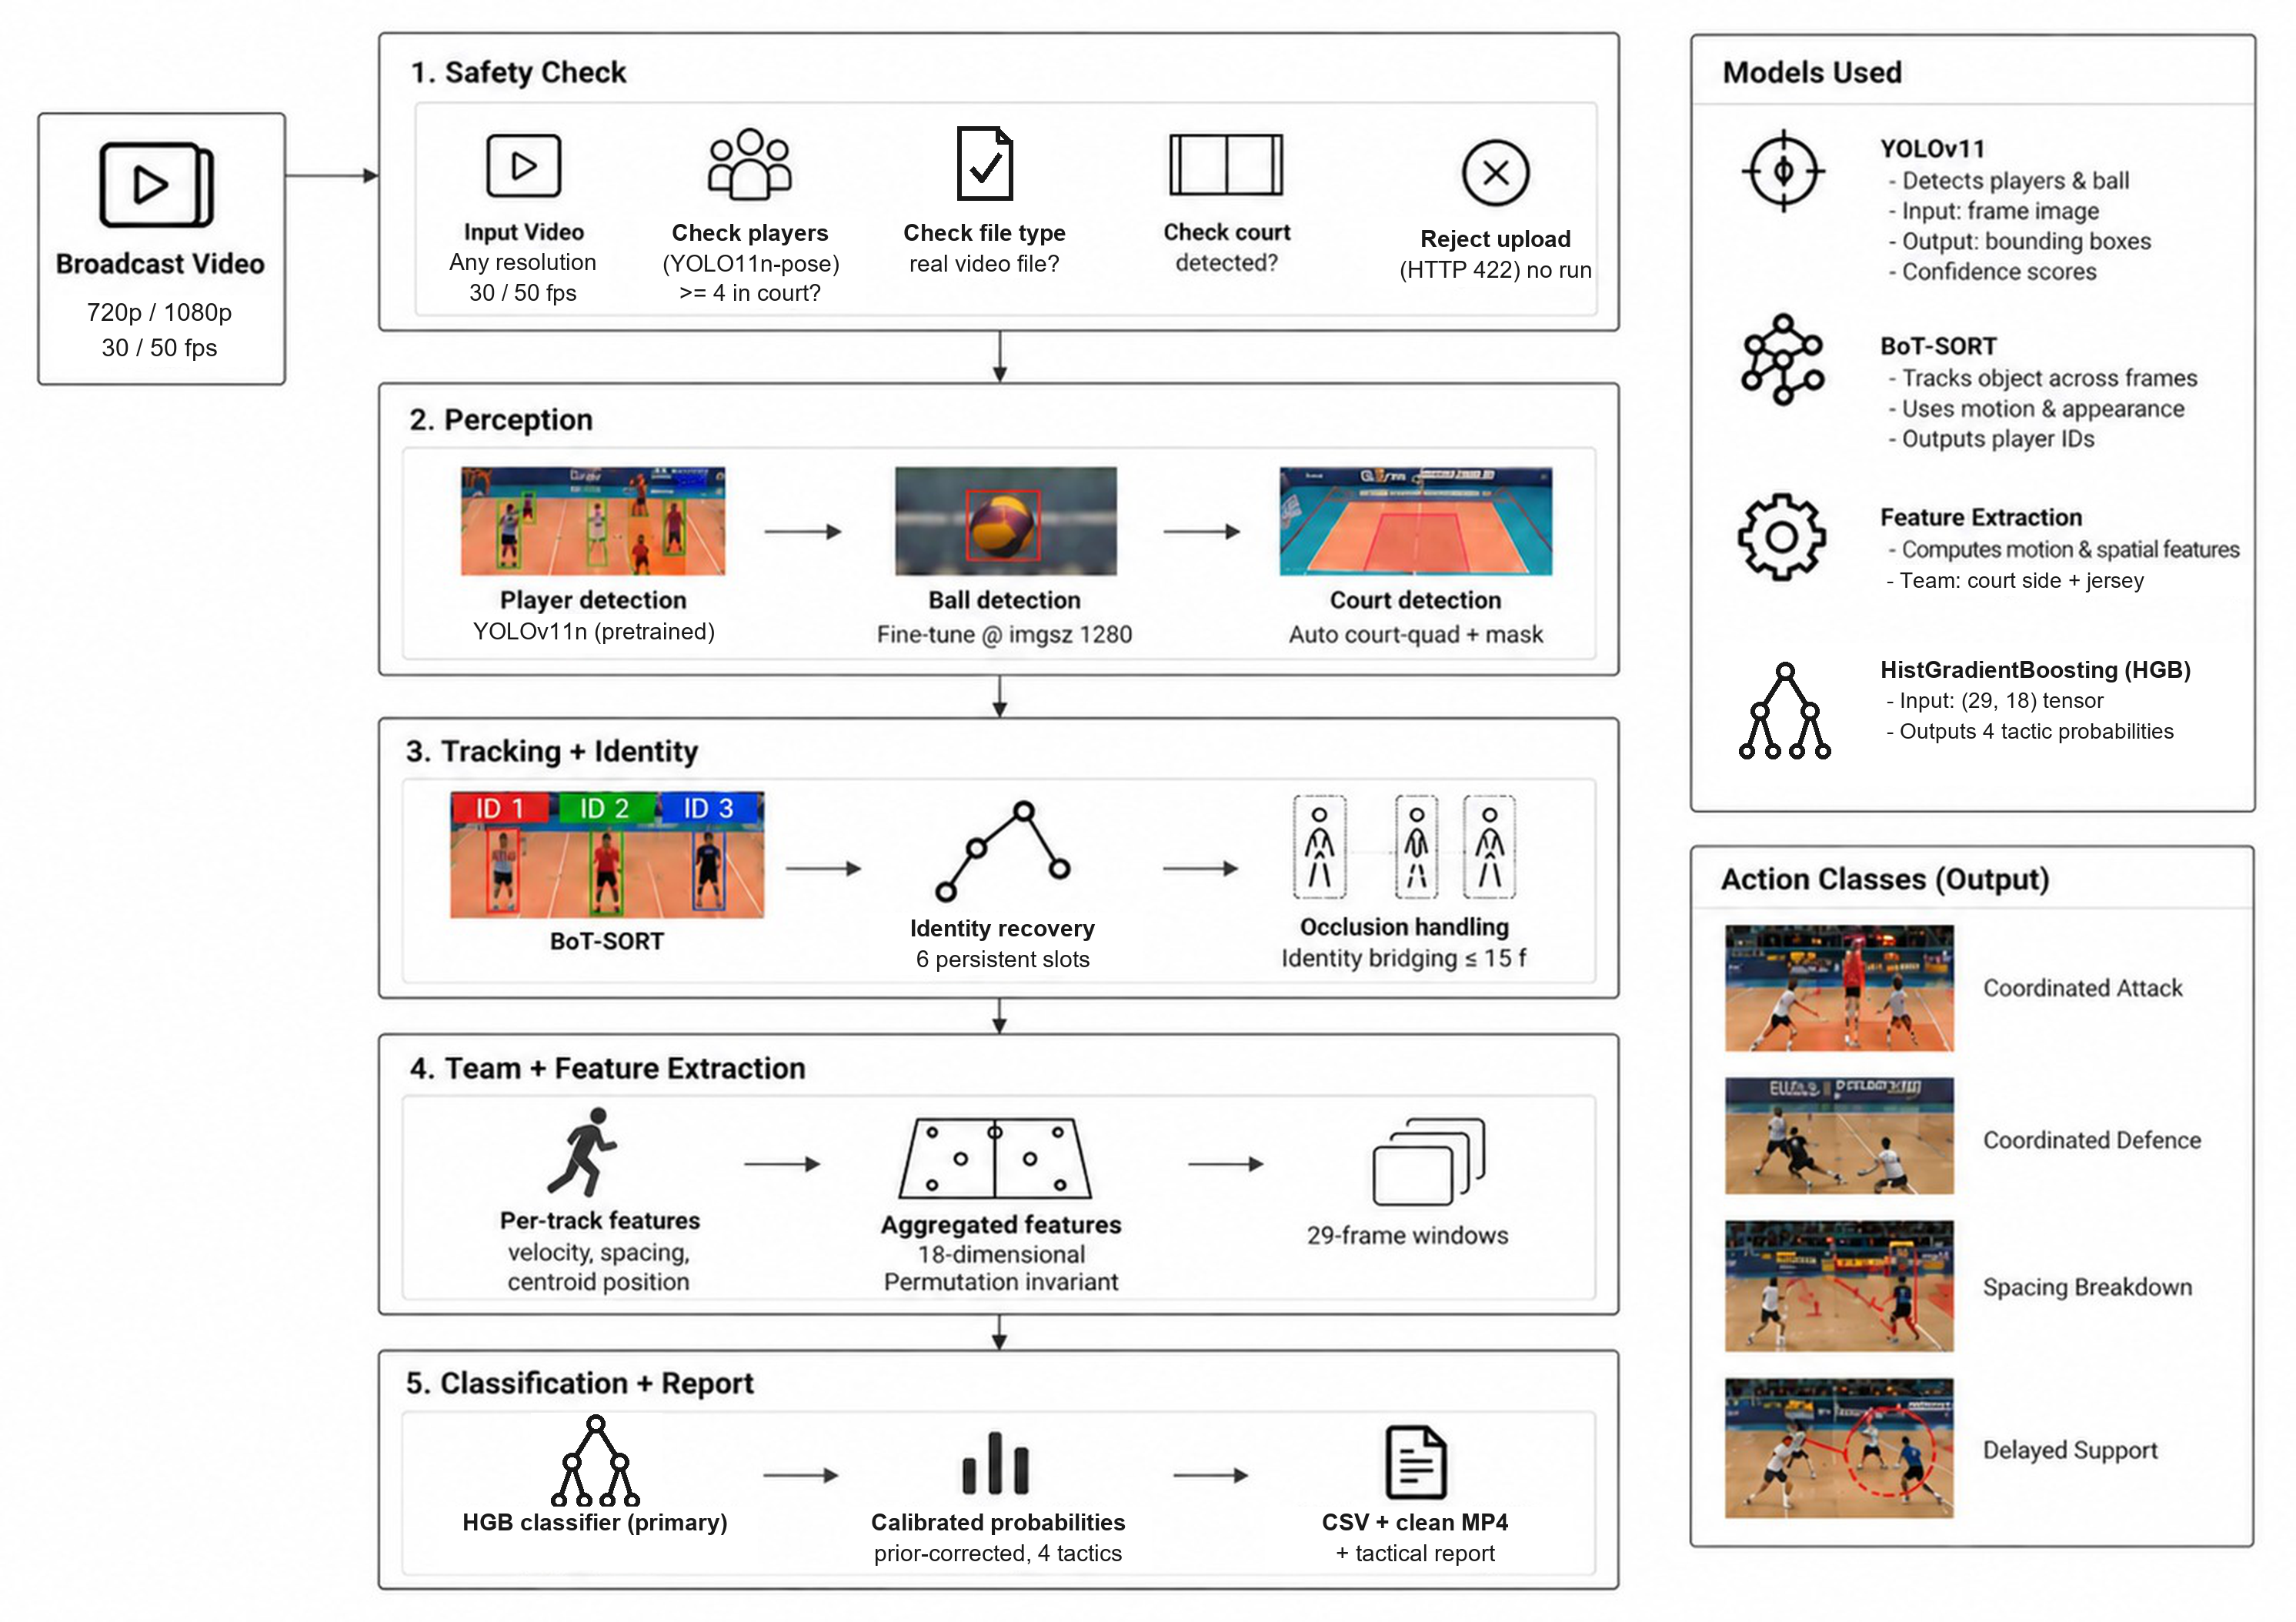
\includegraphics[width=\textwidth]{analysis_pipeline.png}
    \caption{Analysis Pipeline inside the Engine}
\end{figure}

\subsection{Component Design, Data Flow \& Technology Stack}
\begin{itemize}[noitemsep, topsep=2pt]
    \item \textbf{Main Components:} Website (React): the pages the user sees. Server (FastAPI): receives uploads, checks them and manages the job queue. Analysis Engine (Python): does the video analysis. Database (MongoDB): stores the record of every analysis.
    \item \textbf{User Flow:} Home, then Analyze (upload the video, choose the time range and the mode), then Progress, then Results (watch the video, see the tactic timeline, download the reports). A My analyses page lists earlier work.
    \item \textbf{Data Storage \& External Interfaces:} Each analysis has one database record (status and summary) and one folder with the output video, reports and clips. The graphics card (GPU) speeds up player and ball detection, and FFmpeg creates the output videos.
    \item \textbf{Technology Stack:} Python, FastAPI, React, MongoDB, YOLO11 (player and ball detection), scikit-learn (tactic model), OpenCV and FFmpeg (video processing).
\end{itemize}

\section{Implementation Details}

\subsection{Development \& Deployment Environment}
\begin{itemize}[noitemsep, topsep=2pt]
    \item \textbf{Platform \& Runtime Environment:} Windows 11 laptop with an NVIDIA RTX 3050 graphics card. One script (run\_website.bat) starts the database and the server, and the website opens in the browser. A desktop app and a Windows installer are also available.
    \item \textbf{Libraries \& Tools:} FastAPI, React, MongoDB, Ultralytics YOLO11, PyTorch, scikit-learn, OpenCV, FFmpeg and pytest (for automated testing).
    \item \textbf{Source Code Repository:} github.com/Yeshwanthreddy7/volleyball-tactical-intelligence-fyp (version 1.0.0, with documentation and automated tests).
\end{itemize}

\subsection{Module-Wise Implementation \& Integration Summary}
\begin{table}[H]
    \centering
    \footnotesize
    \renewcommand{\arraystretch}{1.25}
    \begin{tabular}{|p{3.5cm}|p{7.8cm}|c|}
        \hline
        \textbf{Application Module} & \textbf{Implemented Features \& Integration Details} & \textbf{Status} \\
        \hline
        Module 1: User Interface & Home, Analyze, Progress, Results, My analyses, Demos, Methodology, Documentation and Team pages; desktop app. & Complete \\
        \hline
        Module 2: Core Analysis & Video check, player and ball detection, player tracking, team separation, tactic model, opponent action detection, annotated video, reports and clips. & Working; known accuracy limits \\
        \hline
        Module 3: Data \& Storage & A database record and a folder for every analysis; old analyses are deleted automatically after 14 days. & Complete \\
        \hline
        Module 4: External Integration & Graphics card (GPU) for fast detection, FFmpeg for video, public project website. & Complete (GPU cloud: future) \\
        \hline
    \end{tabular}
    \caption{Application Module Implementation and Integration Status}
\end{table}

\subsection{Detailed Module Descriptions}
\begin{itemize}[noitemsep, topsep=2pt]
    \item \textbf{User Interface:} The Analyze page lets the user pick a video, the part to analyse and the mode (Accurate or Fast), and shows the upload progress. The Results page plays the annotated video and lists every tactic with its time.
    \item \textbf{Upload \& Video Check:} Only video files (MP4, MOV, AVI, MKV, WebM) are accepted. Before the analysis, the server looks at a few frames to confirm that a volleyball court with players is visible; if not, it shows a clear message.
    \item \textbf{Analysis Engine:} A YOLO11 detector finds the players, and a second detector trained for volleyball finds the ball. A tracker keeps the same ID on each player across frames. The court mapping tells which side of the net each player stands on, which separates the two teams even when the shirts look alike. For the near-side team, the engine measures how spread out the players are, how fast they move and where the ball is, one second at a time, and the trained model (HGB) names the tactic. Moments without live play, such as replays, are skipped. The opponent's serves, spikes and blocks are found with simple rules based on ball touches and body pose.
    \item \textbf{Results \& Reports:} The engine makes the annotated video with the original sound in several qualities, writes the tactic and opponent reports (TXT, CSV and JSON), and cuts short example clips of each tactic.
    \item \textbf{End-to-End Integration:} The website, server, worker, analysis engine and database are fully connected, and each part can be restarted on its own. The same code runs on the laptop and on a cloud server.
\end{itemize}

\section{Functional Testing \& Prototype Demonstration}

\subsection{Functional Test Cases \& Verification}
\begin{table}[H]
    \centering
    \footnotesize
    \renewcommand{\arraystretch}{1.25}
    \begin{tabular}{|p{3.2cm}|p{3.6cm}|p{5.6cm}|c|}
        \hline
        \textbf{Test Case / Feature} & \textbf{Input / User Action} & \textbf{Observed Output} & \textbf{Result} \\
        \hline
        TC-01: Full analysis & 150-second match video, Accurate mode & annotated video, 40 timed tactic segments, 9 opponent actions, example clips for all 4 tactics & Pass \\
        \hline
        TC-02: Video check (real match) & all 11 match videos in our dataset & all accepted & Pass \\
        \hline
        TC-03: Video check (not volleyball) & street photo, test pattern, screen recording & refused with a clear message & Pass \\
        \hline
        TC-04: Wrong file type & a PDF document & refused; the allowed file types are shown & Pass \\
        \hline
        TC-05: Fake video file & a text file renamed to .mp4 & detected and refused & Pass \\
        \hline
        TC-06: File too large & a 5 GB file & refused before the upload starts & Pass \\
        \hline
        TC-07: Security check & request for a missing analysis and for a hidden server file & refused; nothing shown & Pass \\
        \hline
        TC-07b: Cross-user security & a second browser tries to list, cancel, delete or upload into another user's analysis & hidden or refused (403 / 404) in all 6 checks & Pass \\
        \hline
        TC-08: Automated tests & 266 automatic code checks & all 266 passed & Pass \\
        \hline
    \end{tabular}
    \caption{Functional Testing Summary Across Core Application Scenarios}
\end{table}

\subsection{Working Prototype Demonstration}
\begin{figure}[H]
    \centering
    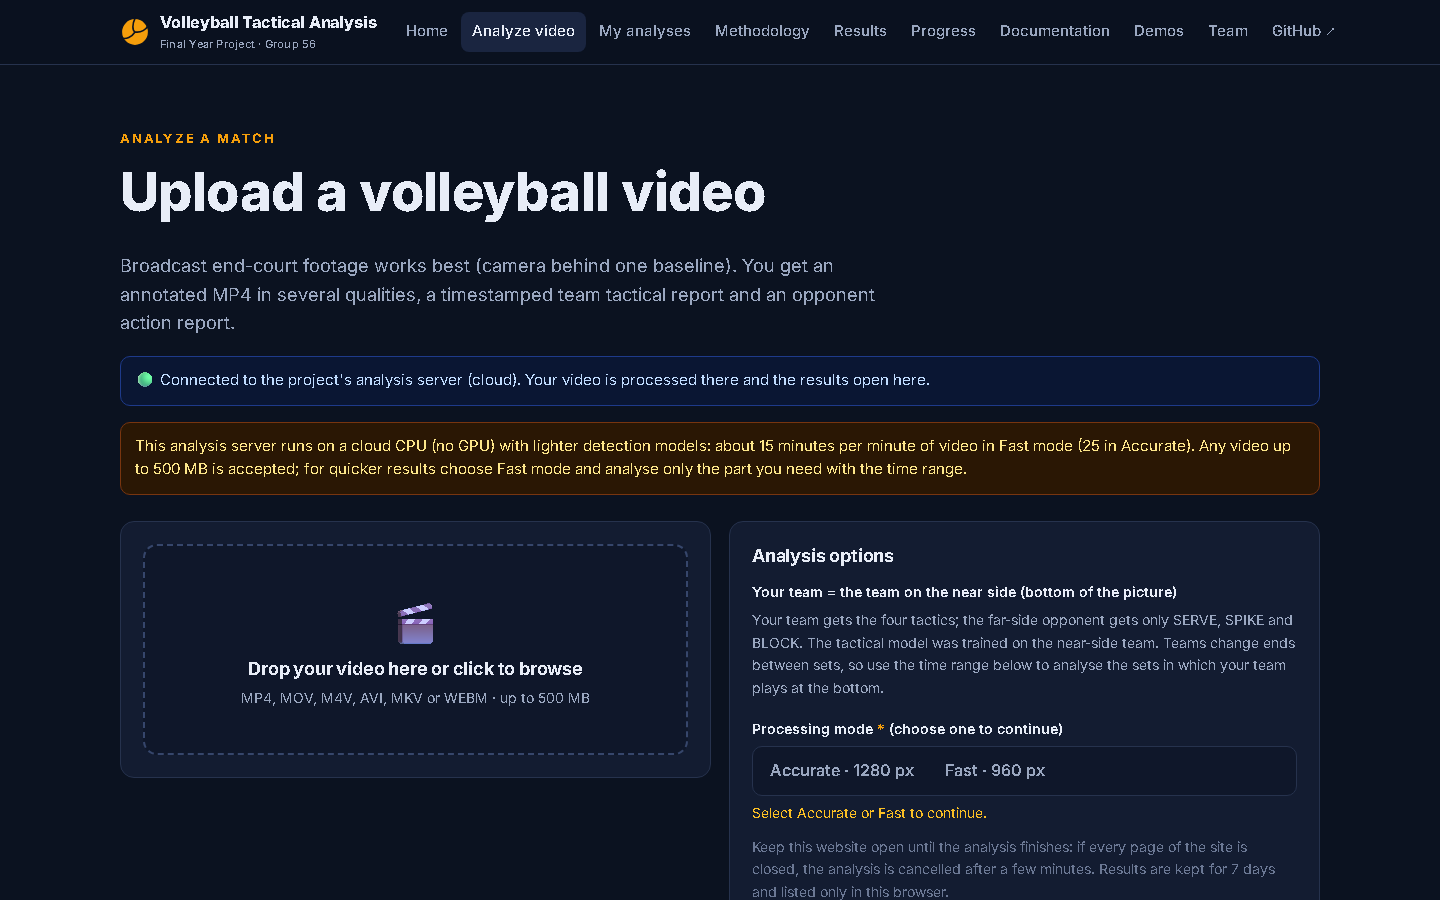
\includegraphics[width=0.49\textwidth]{site_analyze.png}\hfill
    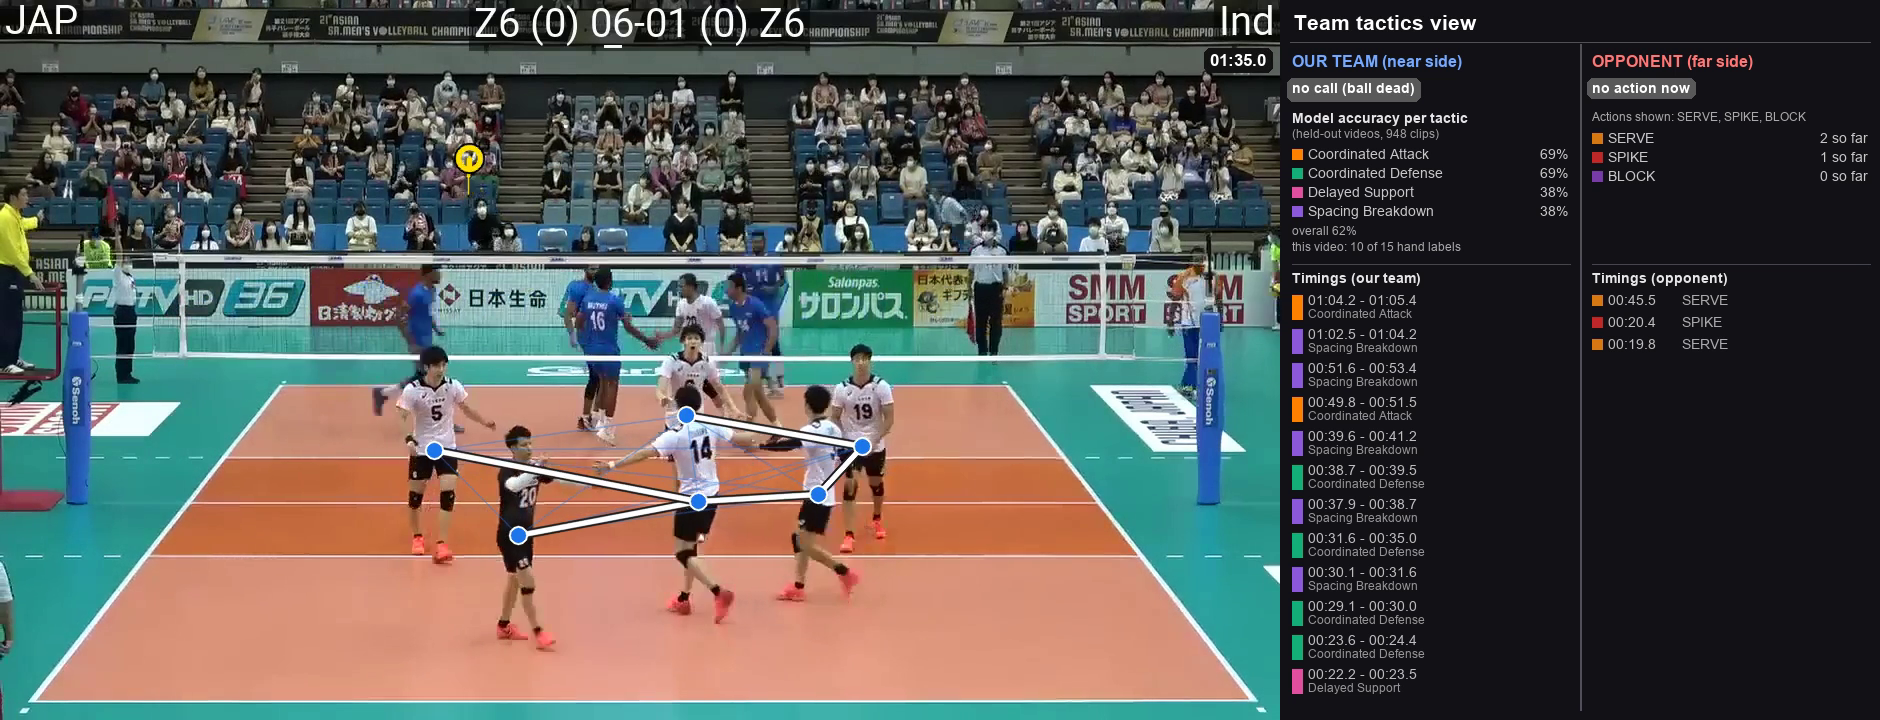
\includegraphics[width=0.49\textwidth]{output_frame.png}
    \caption{Working Prototype: upload page (left) and annotated output video (right)}
\end{figure}

\noindent
\textbf{Evaluation \& Usability Summary:} All test cases passed, including 6 cross-user security checks (evidence/functional\_tests.json). Three full analyses of 1 to 2.5 minutes of match video finished on the laptop and produced every output. On the laptop's graphics card, one minute of 1080p video takes about 7 minutes to analyse, so the tool is meant for review after a match, not for live use. To measure accuracy fairly, the model was trained on 7 match videos and tested on the 8th, and this was repeated for all 8 videos (945 labelled one-second clips). Table 4 compares our model with other models tested in the same way. On the same folds, macro-F1 is 0.54 and weighted-F1 0.66; Attack and Defense reach F1 of about 0.77, while Delayed Support and Spacing Breakdown reach about 0.3 and are mostly confused with each other. InceptionTime and HGB are statistically tied (Wilcoxon over the 8 videos, p = 0.11); HGB is better on 6 of 8 videos. Player tracking reaches IDF1 0.70 on hand-labelled boxes, and court calibration predicts a hidden court line within a median of 5 cm (evidence/*.json).

\begin{table}[H]
    \centering
    \footnotesize
    \renewcommand{\arraystretch}{1.2}
    \begin{tabular}{|l|l|r|}
        \hline
        \textbf{Model} & \textbf{Type} & \textbf{Correct Tactic} \\
        \hline
        HGB, our model (used in the app) & Machine learning & 63.7\% \\
        \hline
        InceptionTime & Deep learning & 61.9\% \\
        \hline
        Mamba & Deep learning & 46.1\% \\
        \hline
        Always guessing the most common tactic & Baseline & 39.0\% \\
        \hline
    \end{tabular}
    \caption{Accuracy on match videos the model never saw during training (945 clips from 8 videos)}
\end{table}

\section{Technical Justification \& Architectural Decisions}
\begin{itemize}[noitemsep, topsep=2pt]
    \item \textbf{Technology Choice:} Python is the standard language for video analysis and machine learning. FastAPI handles large video uploads well, React gives a fast and simple website, and MongoDB stores job records easily. For the tactic model we compared 16 models. HGB was as accurate as the best of them, suits the amount of data we have, and runs fast even without a graphics card, so we chose it over deep-learning models.
    \item \textbf{Design Trade-offs:} The server runs one analysis at a time, so the laptop's graphics card does not run out of memory; other jobs wait in the queue. The analysis runs separately from the website, so a problem in one analysis does not stop the website. Fast mode gives quicker results; Accurate mode finds the small ball more often.
    \item \textbf{Security \& Error Handling:} Only real video files are accepted. A user's analyses can be cancelled or deleted only by that user. Requests for anything other than a real result file are refused. If the user closes the page, the unfinished analysis is stopped after 5 minutes. If the court lines cannot be found, a standard court layout is used. The website has no passwords: each browser gets a random secret ID, stored only as a hash, and another browser cannot see or change its analyses.
    \item \textbf{Deployment:} Today the public website runs on an Azure cloud server without a graphics card (Fast mode), and the laptop with an RTX 3050 runs Accurate mode. A cloud server with a graphics card is future work.
\end{itemize}

\section{Conclusion, Limitations \& Future Scope}
\begin{itemize}[noitemsep, topsep=2pt]
    \item \textbf{Conclusion:} The application works end to end: it accepts an ordinary match video, finds and follows the players and the ball, names the near-side team's tactic every second, and returns an annotated video and reports through a working website. The functional requirements are met. Accuracy is established for Coordinated Attack and Defense (F1 about 0.77 on unseen matches) but not yet for the two rare classes, and the opponent SERVE / SPIKE / BLOCK rules were right in 17 of 31 hand-checked events, so these parts still need more labelled data.
    \item \textbf{Current Limitations:} The analysis is done after the match, not live (about 7 minutes per minute of video). Tactics are given for the team on the near side of the court; because teams change sides between sets, the user analyses one set at a time. The two less common tactics, Delayed Support and Spacing Breakdown, are recognised less reliably than attack and defense. The model was trained on 945 clips from 8 match videos, so more data would improve it. The labels come from one annotator, so no agreement score exists yet. Missed opponent actions and full ball-detection mAP are not measured, because no frame-level hand labels exist. Usefulness to coaches has not been tested with real coaches yet.
    \item \textbf{Future Enhancements:} Run the website on a cloud server with a graphics card for faster results. Add more match videos and labels to improve accuracy. Improve ball detection (a new ball detector is being trained). Recognise team names and follow the same team across sets.
\end{itemize}

\section{Project Deliverables \& Technical Enrichment Summary}
\begin{table}[H]
    \centering
    \footnotesize
    \renewcommand{\arraystretch}{1.2}
    \begin{tabular}{|p{4.2cm}|p{8.6cm}|c|}
        \hline
        \textbf{Deliverable Category} & \textbf{Details / Title / Repository Link} & \textbf{Status} \\
        \hline
        Source Code Repository & github.com/Yeshwanthreddy7/volleyball-tactical-intelligence-fyp; documentation, 266 automated tests, version 1.0.0 & Completed \\
        \hline
        Working Application & Website running on the laptop, desktop app and Windows installer & Completed \\
        \hline
        Individual Online Certifications & G. Bharath Chandra: Python for Computer Vision with OpenCV and Deep Learning (Udemy, 10 h); K. Surya Sekhar: Computer Vision Basics (Coursera (University at Buffalo), 12 h); Keshavramprakash D.: Master Computer Vision: OpenCV4 in Python with Deep Learning (Coursera, 16 h); U. Yeshwanth Kumar Reddy: Python for Computer Vision with OpenCV and Deep Learning (Udemy, 10 h); V. Punith Sai: Python for Computer Vision with OpenCV and Deep Learning (Udemy, 10 h) & Completed \\
        \hline
        Group TEA Deliverable 1 & Project-specific dataset release: Volleyball Backcourt View Dataset on IEEE DataPort, \url{https://ieee-dataport.org/documents/volleyball-backcourt-view-dataset} & Completed \\
        \hline
        Group TEA Deliverable 2 & Project website (Hugging Face Space): \url{https://huggingface.co/spaces/yeshwanthkumarreddy/volleyball-tactical-analysis} & Completed \\
        \hline
        Group TEA Deliverable 3 & Open-source repository: \url{https://github.com/Yeshwanthreddy7/volleyball-tactical-intelligence-fyp.git} & Completed \\
        \hline
    \end{tabular}
    \caption{Summary of Completed Project and Technical Enrichment Deliverables}
\end{table}

\vspace{0.2cm}
\nocite{*}
\renewcommand{\refname}{\large\bfseries\color{amritaMaroon}References}
\bibliographystyle{ieeetr}
\bibliography{ref}

\end{document}
